% !TEX program = latex
% !TEX encoding = UTF-8 Unicode
% !TEX input = Report.tex
% !TEX output = Report.pdf

\documentclass{article}



\usepackage[table]{xcolor}
\usepackage{xcolor}
\usepackage{color,listings}

\usepackage{svg}


\usepackage{array}

\usepackage{mathtools}

\usepackage{pgfplots}
\pgfplotsset{compat=1.15}
\usepackage{mathrsfs}
\usetikzlibrary{arrows}
\pagestyle{empty}

\usepackage{multicol}


\newcommand{\red}{\cellcolor{red!25}}
\newcommand{\blue}{\cellcolor{blue!25}}

\usepackage[left=1in, right=1in, top=1in, bottom=1in]{geometry}

\newcommand{\textbigl}[1]{$\Bigg#1$\nobreak}
\newcommand{\textbigr}[1]{\nobreak$\Bigg#1$}

\newcommand*{\tabbox}[2][t]{
    \vspace{0pt}\parbox[#1][3.7\baselineskip]{1cm}{\strut#2\strut}
}

\usepackage{graphicx}
\graphicspath{ {./} }
\usepackage[font=small,labelfont=bf]{caption}

\usepackage{xcolor}

\usepackage{multirow}

\usepackage{tikz}
\usetikzlibrary{matrix,fit, positioning}

\usepackage{array}
\newcommand{\PreserveBackslash}[1]{\let\temp=\\#1\let\\=\temp}
\newcolumntype{C}[1]{>{\PreserveBackslash\centering}p{#1}}
\newcolumntype{R}[1]{>{\PreserveBackslash\raggedleft}p{#1}}
\newcolumntype{L}[1]{>{\PreserveBackslash\raggedright}p{#1}}

\definecolor{codegreen}{rgb}{0,0.6,0}
\definecolor{codegray}{rgb}{0.5,0.5,0.5}
\definecolor{codepurple}{rgb}{0.58,0,0.82}

\lstdefinestyle{customc}{
    language={C++},
    frame=L,
    xleftmargin=\parindent,
    commentstyle=\color{codegreen},
    keywordstyle=\color{magenta},
    stringstyle=\color{codepurple},
    basicstyle=\ttfamily\footnotesize,
    captionpos=b,                    
    keepspaces=true,                                  
    showspaces=false,                
    showstringspaces=false,
    showtabs=false,
    tabsize=2
}


\lstdefinestyle{lua}{
    language={[5.1]Lua},
    frame=L,
    xleftmargin=\parindent,
    commentstyle=\color{codegreen},
    keywordstyle=\color{magenta},
    stringstyle=\color{codepurple},
    basicstyle=\ttfamily\footnotesize,
    captionpos=b,                    
    keepspaces=true,                                  
    showspaces=false,                
    showstringspaces=false,
    showtabs=false,
    tabsize=2
}

\lstset{escapechar=@,style=customc}

\usepackage{fancyhdr}
\pagestyle{fancy}

\fancyhead[L]{
AI project - Community detection - Genetic
}

\begin{document}
\section*{Introduction}
From point of view of this document, the problem is just to maximize the $Q$ function according to a given graph by partitioning the vertices of the graph. Maximizing $Q$ means to minimize inter-group edges meanwhile inner-group edges are maximized. In this text, we are using the simple genetic algorithm to achieve the goal. For the rest of the document chromosome means the following structure:

\begin{center}
\begin{table}[h]
\begin{tabular}{|c|C{5cm}|c|}
\hline
\multicolumn{3}{|c|}{p: as number of groups} \\\hline
$x_1$: the group which $v_1$ belongs to & $\cdots$ & $x_n$: the group which $v_n$ belongs to\\\hline
\end{tabular}
\end{table}
\end{center}

The maximum number of possible groups is equal to the number of vertices, $n$, therefore we label groups as $0, \dots, n - 1$, which lower group number corresponds to the higher frequent group. If you are asking why the last condition is necessary, it is explained later. After defining the chromosome we modify the main genetic operations, e.g. mutation and etc ..., according to the chromosome and problem structure.

\section*{Code Detail}
There is some useful information about implementation detail for the mentioned operations.
For each operation, three distinct explanation approaches, natural English, Input-Output, Pseducode, are provided. That's enough to understand all the details but you can have a look at the actual code in the given path. 

\subsection*{Initiation}
To create a random initial chromosome we just assign each vertex to a random group from $0, \dots, n - 1$. After that, we do normalize the Chromosome, which means to reorder group numbers to put most larger groups at the first indices.

The code that is used for this purpose is something like this: 

\begin{itemize}

\item Input

\item Output

Chromosome
\textbigl(
\begin{tabular}{|C{2cm}|c|C{2cm}|}
\hline
\multicolumn{3}{|l|}{p = number of vertics} \\\hline
$\cdots$ & $x_i$ = a random number from $0$ to $n - 1$ & $\cdots$ \\\hline
\end{tabular}
\textbigr)

\item Pseudocode
\begin{lstlisting}[style=lua]
function randomChromosome()
	let x be a new chromosome
	for i in 0 ... n do
		x.genome[i] = a random number from 0 ... n - 1
	end
	return nomalized x
end

\end{lstlisting}


\item C++ (you can find this on Solution1/Algorithm.cpp)

\begin{lstlisting}
virtual Chromosome *randomChromosome() const override
{
    Chromosome *chromosome = new Chromosome(problem);
    int problemSize = problem->size();
    chromosome->numberOfGroups = problemSize;
    for(int i = 0; i < problemSize; ++i) {
        (*chromosome)[i] = Random::randomInt(0, problemSize - 1);
    }

    this->_normalize(chromosome);
    return chromosome;
}
\end{lstlisting}
\end{itemize}

\subsection*{Mutation}
 We use mutation to remove small groups and merge them into larger groups. We claim that in the initiation new chromosomes have enough distinct groups. It's easy to show that if the degree of a vertex is zero then we are free to place it in an arbitrary group, it will not affect the value of $Q$. Therefore there are at most $n / 2$ distinct groups in the optimal solution. The following graph shows the number of distinct groups in a chromosome drawn from the above random function averaged over $1000$ tests. This shows there are about $6n / 10$ distinct groups in a randomly generated chromosome. (we will contemplate this soon.)

\begin{center}
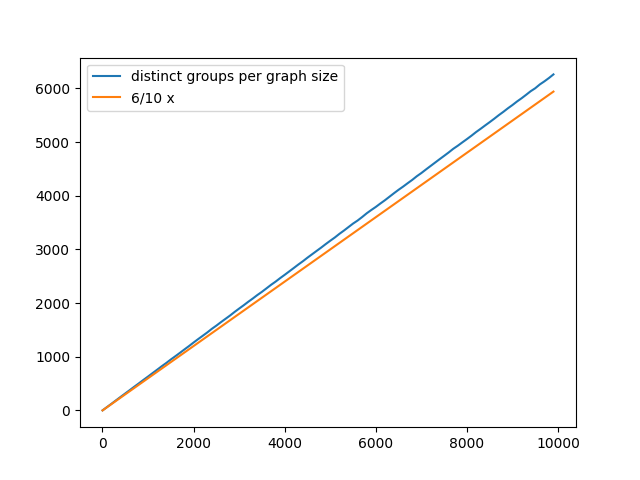
\includegraphics[width=0.49\linewidth]{Figure_1}
\captionof{figure}{Code which generates this graph is placed in numberOfDistinctGroupsInARandomChromosome.py}
\end{center}

It is not hard to proof that expected value of unique values in drawing $n$ numbers from $1$ to $n$  with replacement is equal to 
$
n \times (1 - \left(\frac{n - 1}{n} \right)^n)
$
which converges to $n \times (1 - \frac{1}{e})$ or approximately $n \times 0.63$. Following plot shows  $n \times (1 - \frac{1}{e})$ as red plot and $n \times 0.63$ as purple line. As we can see even in small numbers they are nearly the same.


\definecolor{zzttff}{rgb}{0.6,0.2,1}
\definecolor{ccqqqq}{rgb}{0.8,0,0}
\begin{center}
\begin{tikzpicture}[line cap=round,line join=round,>=triangle 45,x=1cm,y=1cm]
\begin{axis}[
x=1cm,y=1cm,
axis lines=middle,
ymajorgrids=true,
xmajorgrids=true,
xmin=-4.773933675749193,
xmax=7.189034260907393,
ymin=-3.504961316146692,
ymax=4.470350641624318,
xtick={-4,-3,...,7},
ytick={-3,-2,...,4},]
\clip(-4.773933675749193,-3.504961316146692) rectangle (7.189034260907393,4.470350641624318);
\draw[line width=2pt,color=ccqqqq,smooth,samples=100,domain=-4.773933675749193:-6.502457333006365e-8] plot(\x,{(\x)*(1-(((\x)-1)/(\x))^((\x)))});
\draw[line width=2pt,color=ccqqqq,smooth,samples=100,domain=1.0000032187125643:7.189034260907393] plot(\x,{(\x)*(1-(((\x)-1)/(\x))^((\x)))});
\draw[line width=2pt,color=zzttff,smooth,samples=100,domain=-4.773933675749193:7.189034260907393] plot(\x,{0.63*(\x)});
\begin{scriptsize}
\draw[color=ccqqqq] (-4.663845013755421,-2.8505453809614942) node {$f$};
\draw[color=zzttff] (-4.663845013755421,-3.303132102491444) node {$g$};
\end{scriptsize}
\end{axis}
\end{tikzpicture}
\end{center}

As you may notice the number of communities in a graph would be way less than half of the graph vertices. Therefore destroying small groups is reasonable and is suitable for the optimality of the solution. In practice, to do so, we select a random group with the probability of reciprocal of its size and assign its members to other groups randomly.

\newpage
Here we devise an implementation
\begin{itemize}
\item Input

Chromosome
\textbigl(
\begin{tabular}{|c|c|c|}
\hline
\multicolumn{3}{|l|}{p} \\\hline
$x_1$ & $\cdots$ & $x_n$\\\hline
\end{tabular}
\textbigr)

\item Output

Chromosome
\textbigl(
\begin{tabular}{|C{1cm}|p{6.5cm}|C{1cm}|}
\hline
\multicolumn{3}{|c|}{p - 1} \\\hline
\tabbox[b]{$\cdots$} & 
\begin{lstlisting}[style=lua, mathescape=true, frame=none, breaklines=true]
if($x_i$ == a randomly selected group) 
then 
	a random number from 0 ... p - 1
else
	$x_i$
end
\end{lstlisting}
 & \tabbox[b]{$\cdots$} \\\hline
\end{tabular}
\textbigr)

\item Pseudocode
\begin{lstlisting}[style=lua]
function selectGroup(groupsSizes as s)
	c = [ 0 ] -- cumulative sum of 1/s for s in grousp sizes s --
	c[i] = c[i - 1] + 1/s[i] -- s is array of groups sizes --
	
	rc = a random number from [0, last element of c]
	
	return index of first element of c which is greater than or equal to rc
end

function mutate(chromosome)
	s = selectGroup(chromosome.groupSizes)
	for vertex, group in chromosome do
		if(group == s) then
			adj = select a random neighbour of vertex
			if adj == none:
				group = 0 -- if vertex has no adjacent assign it to an special group --
			else 
				group = groups[adj] -- join vertex to the group of one of its adjacents --
			end
		end
	end
end
\end{lstlisting}


\item C++ (you can find this on Solution1/Algorithm.cpp)
\begin{lstlisting}
virtual Chromosome *Algorithm::mutate(const Chromosome *chromosome) const override;
\end{lstlisting}

\end{itemize}

\newpage

\subsection*{Crossover}
In crossover, by definition, we merge two different solution into one in a meaningful way. Here the algorithm is to assign each vertex to the group of corespond vertex in one of its parents randomly. So if we name parents' groups array as $Y$ and $Z$ then $X$ defined as below
\begin{align*}
&x_i = P(u > 0) \times (y_i - z_i) + z_i &&u ~\sim \mathcal{N}(0,\,\sigma^{2})\,.
\end{align*}

In many cases above function will not produce a good result. For example consider following graph

\begin {center}
	\begin {tikzpicture}[-latex ,auto ,node distance = 2cm ,on grid ,
	semithick ,
	first/.style ={ circle ,top color =white , bottom color = blue!20, draw,blue , text=blue , minimum width = 0.5 cm},
	second/.style ={ circle ,top color =white , bottom color = red!20, draw,red , text=red , minimum width = 0.5 cm}
]
	
	\node[first] (A) {$0$};
	\node[first] (B) [below of = A] {$1$};
	\node[first] (C) [right of = B] {$2$};
	\node[first] (D) [right of = A] {$3$};

	\draw[-] (A) -- (B) -- (C) -- (D) -- (A);

	\node[second] (E) [left of = A] {$4$};
	\node[second] (F) [below of = E] {$5$};
	\node[second] (G) [left of = F] {$6$};
	\node[second] (H) [left of = E] {$7$};

	\draw[-] (E) -- (F) -- (G) -- (H) -- (E);

	\end{tikzpicture}
\end{center}

The communities with best $Q$ are shown with different colors. Now consider following chromosomes

\setlength\arraycolsep{20pt}
\[
\begin{array}{cc}
X = \left(
\begin{tabular}{|c|c|c|c|c|c|c|c|}
\hline
\multicolumn{8}{|l|}{p = 2} \\\hline
 0 & 1 & 2 & 3 & 4 & 5 & 6 & 7 \\
\blue 0 & \blue 0 & \blue 0 & \blue 0 &  \blue 0 & \red 1 &  \red 1 & \red 1\\\hline
\end{tabular}
\right)
&
Y = \left(
\begin{tabular}{|c|c|c|c|c|c|c|c|}
\hline
\multicolumn{8}{|l|}{p = 2} \\\hline
 0 & 1 & 2 & 3 & 4 & 5 & 6 & 7 \\
\red 1 & \red 1 & \red 1 & \blue 0 &  \blue 0 & \blue  0 & \blue 0 & \blue 0\\\hline
\end{tabular}
\right)
\end{array}
\]


These solution are close to optimal solution therefore we expect the child solution after crossover be almost optimal but the result is following chromosome.

\begin{center}
\begin{tabular}{m{5.5cm}|m{7cm}}
\hline
\multicolumn{1}{c|}{Chromosome} & \multicolumn{1}{c}{Graph} \\\hline
$
\left(
\begin{tabular}{|c|c|c|c|c|c|c|c|}
\hline
\multicolumn{8}{|l|}{p = 2} \\\hline
 0 & 1 & 2 & 3 & 4 & 5 & 6 & 7 \\
\blue 1 & \red 0 & \blue 1 & \red 0 &  \red 0 & \blue  1 & \blue 1 & \red 0\\\hline
\end{tabular}
\right)
$
&
\begin {tikzpicture}[-latex ,auto ,node distance = 2cm ,on grid ,
semithick ,
first/.style ={ circle ,top color =white , bottom color = blue!20, draw,blue , text=blue , minimum width = 0.5 cm},
second/.style ={ circle ,top color =white , bottom color = red!20, draw,red , text=red , minimum width = 0.5 cm}
]

\node[first] (A) {$0$};
\node[second] (B) [below of = A] {$1$};
\node[first] (C) [right of = B] {$2$};
\node[second] (D) [right of = A] {$3$};

\draw[-] (A) -- (B) -- (C) -- (D) -- (A);

\node[first] (E) [left of = A] {$4$};
\node[second] (F) [below of = E] {$5$};
\node[second] (G) [left of = F] {$6$};
\node[first] (H) [left of = E] {$7$};

\draw[-] (E) -- (F) -- (G) -- (H) -- (E);
\end{tikzpicture}
\end{tabular}
\end{center}
And  one can be see that in general in this approach result chromosome is random and hardly related to it's parents. This problem is caused by different group numbers, and because of this, we should reorder group numbers based on a property to keep crossover effective. Here we reorder groups according to their vertices. This reordering follows only one rule:

\begin{center}
If the smallest vertex of group $a$ is less than that of $b$ then label of $a$ should be less than $b$.
\end{center}

Throughout this document, this reordering is called normalizing and after each operation, each chromosome undergoes this normalization.

Now after this operation $X$ and $Y$ are as follow.
\setlength\arraycolsep{20pt}
\[
\begin{array}{cc}
X = \left(
\begin{tabular}{|c|c|c|c|c|c|c|c|}
\hline
\multicolumn{8}{|l|}{p = 2} \\\hline
 0 & 1 & 2 & 3 & 4 & 5 & 6 & 7 \\
\blue 0 & \blue 0 & \blue 0 & \blue 0 &  \blue 0 & \red 1 &  \red 1 & \red 1\\\hline
\end{tabular}
\right)
&
Y = \left(
\begin{tabular}{|c|c|c|c|c|c|c|c|}
\hline
\multicolumn{8}{|l|}{p = 2} \\\hline
 0 & 1 & 2 & 3 & 4 & 5 & 6 & 7 \\
\blue 0 & \blue 0 & \blue 0 & \red 1 &  \red 1 & \red 1 &  \red 1 & \red 1\\\hline
\end{tabular}
\right)
\end{array}
\]

If we run crossover again the result would be one of the following chromosomes(with same probability), which are way better and more related to the parents than the previous result.

\[
\begin{array}{cc}

Z_{00} = \left(
\begin{tabular}{|c|c|c|c|c|c|c|c|}
\hline
\multicolumn{8}{|l|}{p = 2} \\\hline
 0 & 1 & 2 & 3 & 4 & 5 & 6 & 7 \\
\blue 0 & \blue 0 & \blue 0 & \blue 0 &  \blue 0 & \red 1 &  \red 1 & \red 1\\\hline
\end{tabular}
\right)

&

Z_{01} = \left(
\begin{tabular}{|c|c|c|c|c|c|c|c|}
\hline
\multicolumn{8}{|l|}{p = 2} \\\hline
 0 & 1 & 2 & 3 & 4 & 5 & 6 & 7 \\
\blue 0 & \blue 0 & \blue 0 & \blue 0 &  \red 1 & \red 1 &  \red 1 & \red 1\\\hline
\end{tabular}
\right)

\\[1cm]

Z_{10} = \left(
\begin{tabular}{|c|c|c|c|c|c|c|c|}
\hline
\multicolumn{8}{|l|}{p = 2} \\\hline
 0 & 1 & 2 & 3 & 4 & 5 & 6 & 7 \\
\blue 0 & \blue 0 & \blue 0 & \red 1 &  \blue 0 & \red 1 &  \red 1 & \red 1\\\hline
\end{tabular}
\right)

&

Z_{11} = \left(
\begin{tabular}{|c|c|c|c|c|c|c|c|}
\hline
\multicolumn{8}{|l|}{p = 2} \\\hline
 0 & 1 & 2 & 3 & 4 & 5 & 6 & 7 \\
\blue 0 & \blue 0 & \blue 0 & \red 1 &  \red 1 & \red 1 &  \red 1 & \red 1\\\hline
\end{tabular}
\right)

\end{array}
\]
\newpage
\begin{itemize}
\item Input

X
\textbigl(
\begin{tabular}{|c|c|c|}
\hline
\multicolumn{3}{|l|}{$p$} \\\hline
$x_1$ & $\cdots$ & $x_n$\\\hline
\end{tabular}
\textbigr)

Y
\textbigl(
\begin{tabular}{|c|c|c|}
\hline
\multicolumn{3}{|l|}{$p^\prime$} \\\hline
$y_1$ & $\cdots$ & $y_n$\\\hline
\end{tabular}
\textbigr)

\item Output

Chromosome
\textbigl(
\begin{tabular}{|C{1cm}|p{6.5cm}|C{1cm}|}
\hline
\multicolumn{3}{|c|}{at most $\max\{p, p^\prime\}$} \\\hline
$\cdots$ & randomly selected from $x_i$ and $y_i$ & $\cdots$ \\\hline
\end{tabular}
\textbigr)

\item Pseudocode
\begin{lstlisting}[style=lua]
function crossover(x, y)
	let z be a new chormosome 

	z.p = max(x.p, y.p)

	for i in 0 ... number of vertices do
		z.genomes[i] = randomInt(0, 1) * (x.genomes[i] - y.genomes[i]) + y.genomes[i]
	end

	return nomalized z
end
\end{lstlisting}


\item C++ (you can find this on Solution1/Algorithm.cpp)
\begin{lstlisting}
virtual Chromosome *crossover(const Chromosome *X, const Chromosome *Y) const override
{
    Chromosome *newChromosome = new Chromosome(problem);
    int problemSize = problem->size();

    newChromosome->numberOfGroups = std::max(X->numberOfGroups, Y->numberOfGroups);

    for(int i = 0; i < problemSize; ++i) {
        if(Random::randomInt(0, 1)) {
            (*newChromosome)[i] = (*X)[i];
        } else {
            (*newChromosome)[i] = (*Y)[i];
        }
    }

    this->_normalize(newChromosome);
    return newChromosome;
}
\end{lstlisting}
\end{itemize}

\newcommand{\bash}[1]{\colorbox{gray!30}{\lstinline{#1}} }

\newpage
\section*{Execution}
\subsection*{Build}
To build project the you can easily use provided MakeFiles by running \bash{make all} or \bash{make win} for windows  in command line, then you can run the code by executing \bash{console.exe} or \bash{console.out}. For compile manually use following command
\begin{lstlisting}
g++ -std=c++20 console.cpp -o console -I.
\end{lstlisting}

\subsection*{Inputs}
The program expects you to put a file name \bash{graph.txt} in the project directory containing graph edges. If file does not exsist program asks for new file name and you can enter \bash{stdin} to enter graph manually.

\subsection*{Outputs}
The program generates some useful logs but the final result will be displayed and be written to a file named \bash{communities.py}. Also, a colored graph is generated in dot format which you can use Graphviz to visualize, this graph is written to \bash{graph.dot}. After running the code you can run script \bash{compareResults.py} to compare this code outputs with \bash{networkx}'s output.

An example of output graph is shown below(using provided the dataset.txt)

\begin{center}
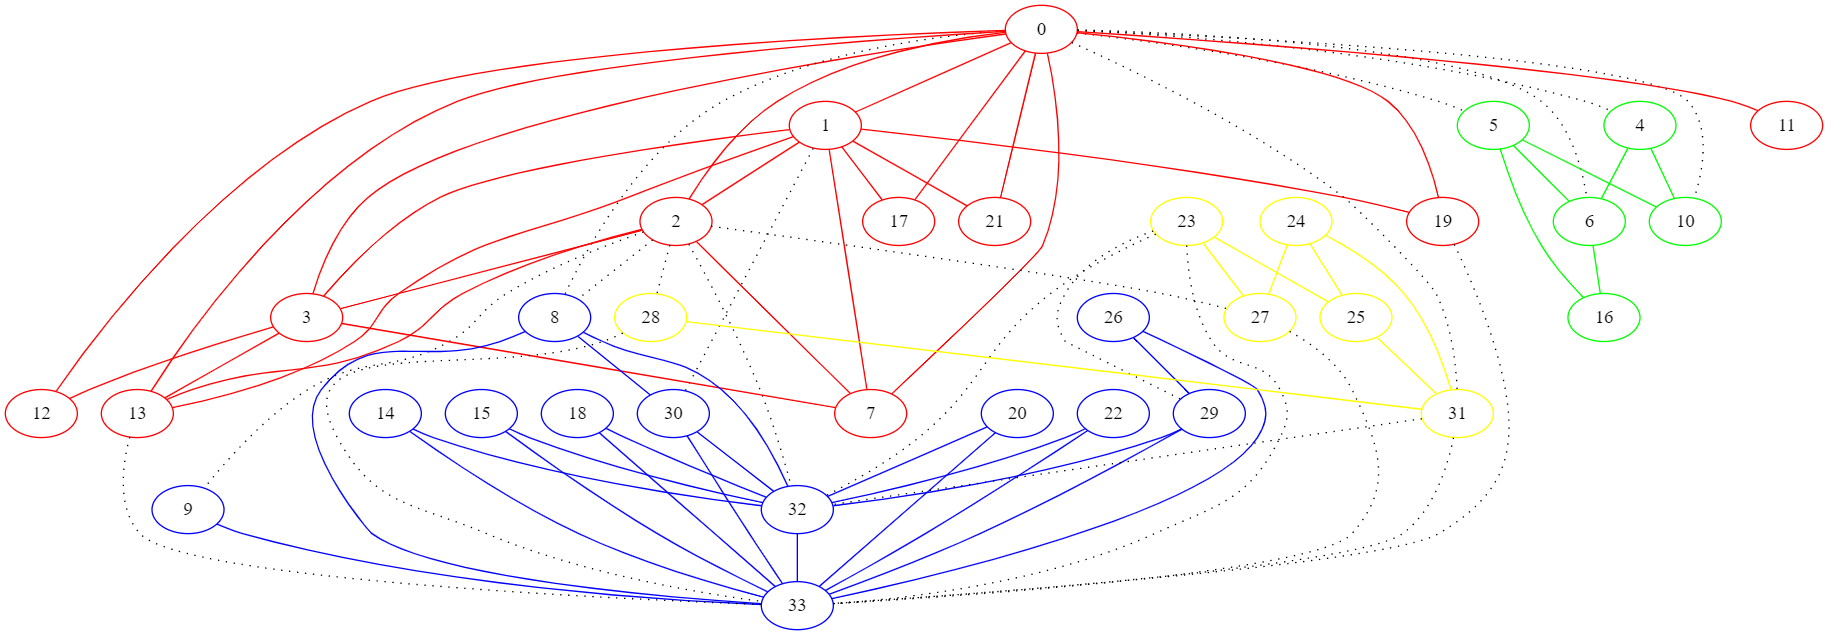
\includegraphics[height=8cm, width=\linewidth]{graphviz}
\end{center}

\end{document}
